\section{Methodology}
 Proposed machine learning approach (e.g., supervised learning, unsupervised learning, deep learning).
    
Algorithms/models under consideration.

Tools, libraries, and frameworks you plan to use.

\begin{figure}[h]
    \centering
    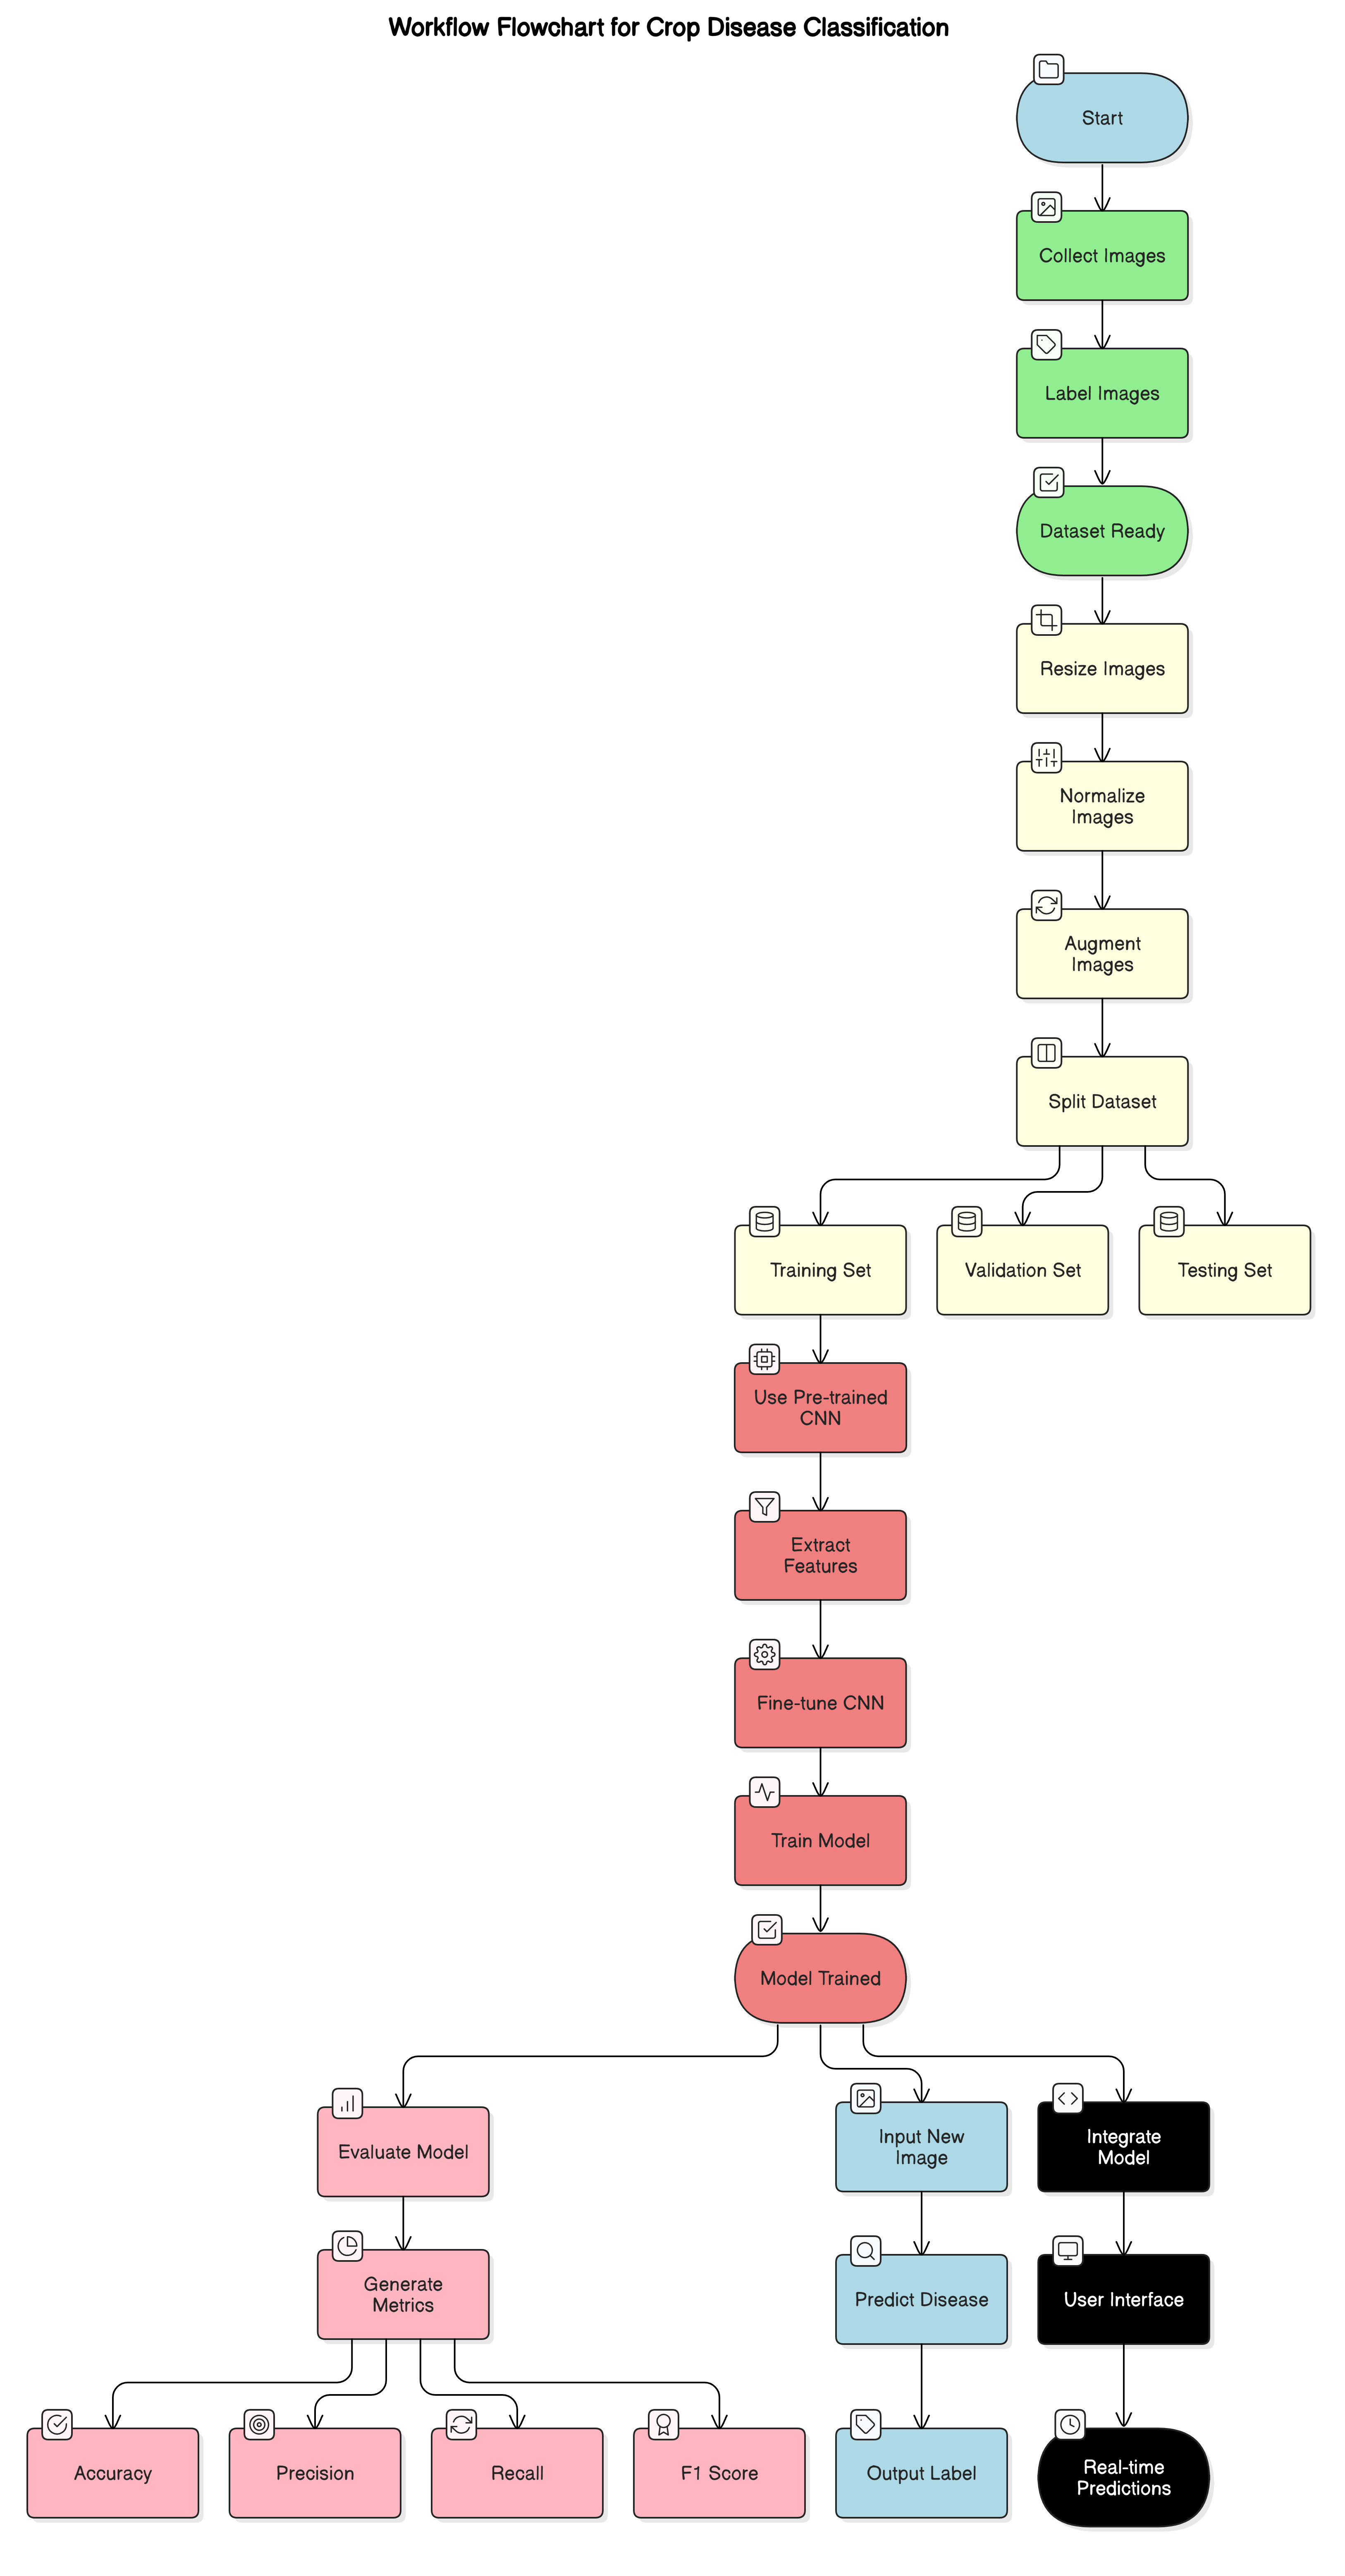
\includegraphics[width=0.5\linewidth]{Images/flow.png}
    \caption{Caption}
    \label{fig:enter-label}
\end{figure}

\begin{table}[h]
    \centering
    \caption{sample Cost-Benefit Analysis of the Proposed Project}
    \begin{tabular}{@{}llcc@{}}
        \toprule
        \textbf{Item} & \textbf{Description} & \textbf{Cost (\$)} & \textbf{Benefit (\$)} \\ \midrule
        Development Costs & Software Development & 15,000 & - \\
        Hardware Costs & Servers and Equipment & 5,000 & - \\
        Training Costs & User Training Sessions & 2,000 & - \\
        Maintenance Costs & Annual Maintenance & 1,000 & - \\
        \midrule
        \textbf{Total Costs} &  & \textbf{23,000} & - \\ \midrule
        Increased Efficiency & Time Savings & - & 30,000 \\
        Improved User Satisfaction & User Feedback & - & 10,000 \\
        Revenue Increase & New Customers & - & 20,000 \\
        \midrule
        \textbf{Total Benefits} &  & - & \textbf{60,000} \\ \midrule
        \textbf{Net Benefit} &  & \textbf{23,000} & \textbf{37,000} \\ 
        \bottomrule
    \end{tabular}
    \label{tab:cost-benefit}
\end{table}

 


\url{https://www.onlinegantt.com/#/gantt} to create a Gantt chart as per our need.
  
